\documentclass[10pt,a4paper,landscape]{article}
\usepackage[a4paper,landscape,margin=12mm,top=11mm,bottom=12mm]{geometry}
\usepackage[T1]{fontenc}
\usepackage{mathptmx}
\usepackage{booktabs,tabularx,array,enumitem,xcolor,graphicx,multicol}
\usepackage[colorlinks=true,citecolor=blue,urlcolor=blue,linkcolor=blue]{hyperref}
\usepackage{cite}
\pagestyle{plain}
\setlength{\parindent}{0pt}\setlength{\parskip}{3pt}
\setlist{nosep,leftmargin=12pt,topsep=2pt}
\newcolumntype{L}{>{\raggedright\arraybackslash}X}
\newcolumntype{P}[1]{>{\raggedright\arraybackslash}p{#1}}
\definecolor{win}{HTML}{1f7a45}\definecolor{lose}{HTML}{b3261e}
\newcommand{\W}{\textcolor{win}{\textbf{better}}}
\newcommand{\Lo}{\textcolor{lose}{\textbf{worse}}}
\renewcommand{\arraystretch}{1.12}
\begin{document}

{\LARGE\bfseries SeizeLUT: comparison with published work and results}\hfill
{\small BISP project, ECE, NIT Warangal, November 2026}\par
{\small Akshara Bonam (23ECB0A11) \quad Sai Chaithr (23ECB0A20) \quad Sowjanya (23ECB0A22)}\par
\vspace{2pt}\hrule\vspace{4pt}

\textbf{How to read this.} Section 1 compares with the SeizeIT2 dataset paper on the \emph{same} 29 test patients
and with its own metrics, so those numbers are directly comparable. Section 2 compares all models we trained, under one
protocol on the same patients. Section 3 lists hardware seizure detectors as their papers report them; they use other
data, other metrics and mostly patient-specific training, so that table shows the design space, not a ranking. All our
numbers come from the held-out test patients (sub-097 to sub-125), scored once after the design was frozen, unless
marked otherwise.

\section*{1. Against the SeizeIT2 dataset paper (same data, same 29 test patients)}

\begin{minipage}[t]{0.56\textwidth}
\vspace{0pt}
\small
\begin{tabularx}{\textwidth}{@{}LP{24mm}P{19mm}P{26mm}@{}}
\toprule
\textbf{Detector} & \textbf{Seizures detected} & \textbf{False alarms per hour} & \textbf{Note}\\
\midrule
SVM, published \cite{bhagubai2025seizeit2} & 71.1\,\% & 11.0 & bte-EEG only\\
ChronoNet, published \cite{bhagubai2025seizeit2} & 84.2\,\% & 100.5 & bte-EEG only\\
ChronoNet, our port, released protocol & 74.5\,\% & 22.6 & picks its epoch on the test patients\\
ChronoNet, our port, clean protocol & 67.1\,\% & 11.9 & no test information\\
\midrule
\textbf{SeizeLUT two-stage} (post-ictal check) & \textbf{73.3\,\%} $\pm$ 1.4 & \textbf{10.9} $\pm$ 0.6 & \W\ than the SVM at a lower FA rate$^{a}$\\
\textbf{SeizeLUT final DWN}, frozen point & 25.5\,\% & \textbf{0.02} & 0.8 false alarms per \emph{day}\\
SeizeLUT final DWN at 1.2 FA/h & \textbf{43.2\,\%} & 1.2 & ChronoNet (clean): 34.8\,\% at 1.2\\
\bottomrule
\end{tabularx}

\vspace{3pt}
{\footnotesize $^{a}$ Pre-registered secondary analysis after the final test (training folds: 81.9\,\% at 9.6); 96-s
decision delay, suited to seizure logging. Window AUROC: SeizeLUT 0.883, ChronoNet 0.746. The published ChronoNet
figure could only be partly reproduced (74.5\,\% vs 84.2\,\%) with a line-by-line port of the released code; its
released protocol selects the model on the test patients, so we report the clean run as the fair reference.}
\end{minipage}\hfill
\begin{minipage}[t]{0.42\textwidth}
\vspace{0pt}
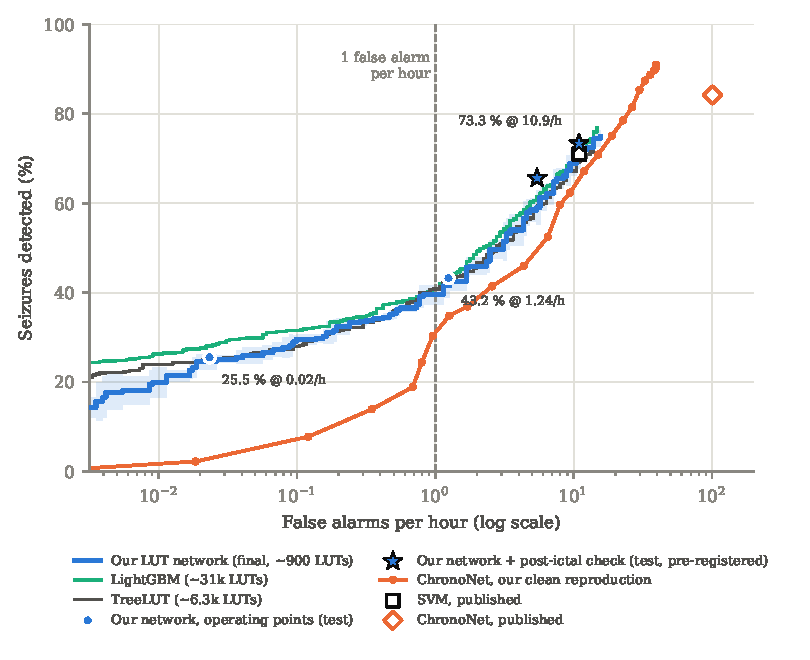
\includegraphics[width=\textwidth]{figures/sens_fa_test.pdf}

{\footnotesize Seizures detected vs false alarms per hour on the 29 test patients (dataset paper's metrics). Curves:
threshold sweeps of the frozen models; dots: operating points chosen on the training folds; stars: two-stage detector;
open markers: published values.}
\end{minipage}

\vspace{4pt}
\textbf{Verdict:} at the dataset paper's own false-alarm rate SeizeLUT detects \textbf{more seizures than the
published SVM}, with a classifier of about 1,200 FPGA lookup tables instead of software; at a low false-alarm rate it
detects more seizures than ChronoNet (43.2\,\% vs 34.8\,\%), and its default setting raises fewer than one false alarm
per day.

\newpage
\section*{2. Against other models on the same 29 test patients (one protocol, 5 seeds)}

\begin{minipage}[t]{0.60\textwidth}
\vspace{0pt}
\small
\begin{tabularx}{\textwidth}{@{}LrrrrP{24mm}@{}}
\toprule
\textbf{Model} & \textbf{Event-F1} & \textbf{Sens.} & \textbf{FA/day} & \textbf{AUROC} & \textbf{Hardware cost}\\
\midrule
\textbf{SeizeLUT: DWN + distillation (final)} & \textbf{0.248} & 0.303 & 0.8 & 0.883 & \textbf{895 LUTs}$^{b}$, no mult.\\
LightGBM (gradient-boosted trees) & 0.308 & 0.331 & 0.6 & 0.877 & 30,750 LUTs\\
XGBoost & 0.294 & 0.301 & 0.4 & 0.872 & 48,295 LUTs\\
CatBoost & 0.254 & 0.330 & 1.2 & 0.874 & 27,720 LUTs\\
Random forest & 0.246 & 0.245 & 0.2 & 0.858 & 346,576 LUTs\\
TreeLUT, 5-bit leaves \cite{khataei2025treelut} & 0.233 & 0.292 & 1.0 & 0.858 & 6,330 LUTs\\
Logic-gate network \cite{petersen2022dlgn} & 0.191 & 0.291 & 1.4 & 0.865 & 7,452 LUTs\\
INT8 MLP & 0.155 & 0.249 & 1.7 & 0.788 & 9,600 multipliers\\
Logistic regression & 0.123 & 0.255 & 5.1 & 0.814 & 117 multipliers\\
ChronoNet, clean \cite{roy2019chrononet} & 0.027 & 0.790 & 106.3 & -- & CNN + GRU\\
\bottomrule
\end{tabularx}

\vspace{3pt}
{\footnotesize SzCORE event scoring \cite{dan2024szcore}, mean over patients, best-F1 operating point chosen on the
training folds. $^{b}$Estimated cost used for the model comparison; the implemented classifier is 398 LUTs in Vivado
(Section 4).}
\end{minipage}\hfill
\begin{minipage}[t]{0.38\textwidth}
\vspace{0pt}
\textbf{What this shows}
\begin{itemize}
\item \textbf{Above} TreeLUT (0.233) with a seventh of its LUTs, above the logic-gate network, the INT8 MLP,
  logistic regression and ChronoNet (per-patient $p = 0.027$).
\item \textbf{Level} with CatBoost and random forest, which need 30 to 390 times more LUTs.
\item \textbf{Below} LightGBM (0.308, $p = 0.039$) and XGBoost, which need about 30,000--48,000 LUTs.
\item Distillation from LightGBM is what lifted the network from 0.172 to 0.248 and cut false alarms from 2.7 to 0.8
  per day.
\item ChronoNet finds most seizures (79\,\%) but raises over 100 false alarms per day.
\end{itemize}
\end{minipage}

\section*{3. Against published hardware seizure detectors (as reported; not directly comparable)}

{\small
\setlength{\tabcolsep}{3pt}
\begin{tabularx}{\textwidth}{@{}P{30mm}P{24mm}P{36mm}P{28mm}P{50mm}P{32mm}P{20mm}L@{}}
\toprule
\textbf{Work} & \textbf{Platform} & \textbf{Data (patients), training} & \textbf{Inputs} & \textbf{Detection (as reported)} &
\textbf{Cost} & \textbf{Energy/inf.} & \textbf{Fault test}\\
\midrule
Altaf 2015 \cite{altaf2015jssc} & ASIC 180\,nm & CHB-MIT (14)$^\ddagger$, PS & EEG, 16 ch & sens 95.7\,\%, spec 98\,\%$^\ddagger$ & 1.56\,mm$^2$/ch$^\ddagger$ & 2.73\,\textmu J$^\ddagger$ & not reported\\
Shoaran 2018 \cite{shoaran2018jetcas} & ASIC 65\,nm & iEEG (26), PS & iEEG & F1 87.9\,\% (block split) & 1.0\,mm$^2$ & 41.2\,nJ & not reported\\
NeuralTree 2022 \cite{shin2022neuraltree} & ASIC 65\,nm & CHB-MIT (24) + iEEG (6), PS & EEG/iEEG, $\le$64 ch & sens 95.6\,\%, spec 96.8\,\% & 3.48\,mm$^2$ & 0.227\,\textmu J & not reported\\
Vittimberga 2025 \cite{vittimberga2025sensors} & Artix-7 (synthesis) & CHB-MIT (5), PS & EEG, 4 ch & sens $>$98\,\% (samples) & 192 LUT, 3 DSP & n.r. & not reported\\
Busia 2025 \cite{busia2025fpga} & iCE40UP5K FPGA & CHB-MIT (9), PS & EEG, 4 ch & 100\,\% of events, 0.3 FA/h & 3.3k LC, 2 DSP, 14 BRAM & 4.55\,nJ (core) & not reported\\
EEGformer 2024 \cite{busia2024eegformer} & GAP9 MCU & CHB-MIT (8), PS & EEG, 4 ch & 73\,\% of events, 0.15 FA/h & 150\,kB, 14.7 MOPS & 0.31\,mJ & not reported\\
BrainFuseNet 2024 \cite{ingolfsson2024brainfusenet} & GAP9 MCU & PEDESITE (6), PS & EEG 4 ch, PPG, ACC & 95\,\% of events, 0.58 FA/day & 2.29 M MAC & 0.11\,mJ & not reported\\
SeizeIT2 2025 \cite{bhagubai2025seizeit2} & software & SeizeIT2 (29 test), PI & bte-EEG, 2 ch & SVM 71.1\,\% at 11.0 FA/h & -- & -- & --\\
\midrule
\textbf{SeizeLUT (ours)} & \textbf{Kria KV260 board} (XCK26) & \textbf{SeizeIT2 (29 test), PI} & bte-EEG 2 ch, ECG, EMG, ACC, GYR &
event-F1 0.248 at 0.8 FA/day; two-stage 73.3\,\% at 10.9 FA/h & 398 LUT, 0 DSP; whole detector 1,202 LUT & $\approx$43\,pJ$^\ast$ &
\textbf{100\,\% of decision-relevant faults; measured on the board}\\
\bottomrule
\end{tabularx}}

{\footnotesize PS: patient-specific training or calibration (tested on the same patients it was tuned for); PI:
patient-independent (tested on unseen patients, much harder). $^\ddagger$From the comparison table of
\cite{shin2022neuraltree}. $^\ast$Vivado vectorless estimate (17\,mW dynamic at 400\,MHz, one window per clock), not
a measurement. Detection metrics differ (event-, epoch- or sample-based). Sources of every number:
\texttt{results/tables/prior\_work\_sources.md}.}

\textbf{Verdict:} the patient-specific detectors report higher accuracy on easier, tuned-per-patient settings; SeizeLUT
is the only one here that is patient-independent on a multimodal wearable dataset, runs on a real board, and checks
its own hardware. Vittimberga 2025 is smaller (192 LUTs plus 3 DSP blocks) but patient-specific, EEG-only, sample-scored
and reported from synthesis only.

\newpage
\section*{4. Against other lookup-table networks on the same FPGA (cost of the classifier)}

\begin{minipage}[t]{0.55\textwidth}
\vspace{0pt}
\small
\begin{tabularx}{\textwidth}{@{}LrrrrrP{14mm}@{}}
\toprule
& \multicolumn{4}{c}{\textbf{Vivado 2026.1, XCK26}} & \textbf{Yosys} & \\
\cmidrule(lr){2-5}
\textbf{Model} & \textbf{LUTs} & \textbf{FFs} & \textbf{Fmax} & \textbf{Dyn.\ power} & \textbf{LUTs} & \textbf{Test F1}\\
\midrule
\textbf{DWN + distillation (ours)} \cite{bacellar2024dwn} & \textbf{398} & 454 & \textbf{468\,MHz} & \textbf{17\,mW} & 405 & \textbf{0.248}\\
TreeLUT, 5-bit leaves \cite{khataei2025treelut} & 2,677 & 1,461 & 294\,MHz & 88\,mW & 2,721 & 0.233\\
Logic-gate network \cite{petersen2022dlgn} & 5,249 & 2,208 & 154\,MHz & 523\,mW & 5,758 & 0.191\\
\bottomrule
\end{tabularx}

\vspace{3pt}
{\footnotesize Out of context, 2.5-ns constraint, vectorless power at 400\,MHz. All three generated from their frozen
final models and checked bit-exact in simulation.}

\vspace{6pt}
\begin{tabularx}{\textwidth}{@{}LP{52mm}@{}}
\toprule
\textbf{Whole detector (ours)} & \textbf{Cost}\\
\midrule
Feature engine (front end in the fabric) & 804 LUTs, 4.5 block RAMs, 0 DSP, 234\,MHz\\
Front end + classifier & \textbf{1,202 LUTs, no multiplier}\\
Full KV260 design (with self-test, fault injection, demo I/O) & 3,796 LUTs (3.2\,\% of the chip); timing met at 100\,MHz\\
\bottomrule
\end{tabularx}
\end{minipage}\hfill
\begin{minipage}[t]{0.42\textwidth}
\vspace{0pt}
\textbf{What this shows}
\begin{itemize}
\item The DWN is \textbf{6.7$\times$ smaller} than TreeLUT and \textbf{13.2$\times$ smaller} than the logic-gate
  network, \textbf{the fastest} of the three, and \textbf{the most accurate} of the three.
\item The two synthesis tools agree (Vivado 398, Yosys 405 LUTs).
\item The whole detector, including the signal processing, is 1,202 LUTs with no multiplier, and it keeps up with the
  sensors at under 1\,MHz.
\end{itemize}
\end{minipage}

\section*{5. Self-test: our selected vectors against the usual choices}

\begin{minipage}[t]{0.55\textwidth}
\vspace{0pt}
\small
\begin{tabularx}{\textwidth}{@{}Lrrrr@{}}
\toprule
\textbf{Self-test vector set} & \textbf{Vectors} & \multicolumn{3}{c}{\textbf{Decision-relevant faults detected}}\\
\cmidrule(lr){3-5}
& & \textbf{Truth-table} & \textbf{Stuck-at} & \textbf{All}\\
\midrule
Consecutive recorded windows (usual golden test) & 1,024 & 43.6\,\% & 94.5\,\%/100\,\% & 50.7\,\%\\
Random training windows & 1,024 & 79.4\,\% & 100\,\% & 82.2\,\%\\
\textbf{Coverage-selected windows (ours)} & \textbf{255} & \textbf{100\,\%} & \textbf{100\,\%} & \textbf{100\,\%}\\
\bottomrule
\end{tabularx}

\vspace{3pt}
{\footnotesize 3,592 single faults (3,200 truth-table flips, 392 stuck-at); 2,890 change a decision on the 8,714
training hours. On the KV260 all 3,592 faults were injected through registers: hardware and software agreed on every
fault; the self-test runs 1,024 vectors in 10.3\,\textmu s. None of the hardware detectors in Section 3 reports a fault
analysis.}
\end{minipage}\hfill
\begin{minipage}[t]{0.42\textwidth}
\vspace{0pt}
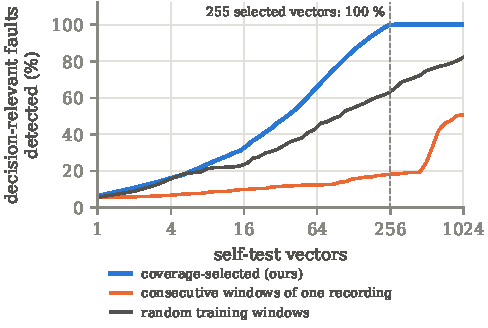
\includegraphics[width=\textwidth]{figures/fault_coverage.pdf}
\end{minipage}

\section*{Summary}
\begin{tabularx}{\textwidth}{@{}P{55mm}L@{}}
\toprule
\textbf{Where SeizeLUT is better} & more seizures than the dataset paper's SVM at its false-alarm rate (73.3\,\% vs 71.1\,\%);
far fewer false alarms than all published SeizeIT2 baselines (0.8 per day); of the three lookup-table networks the smallest, fastest and most accurate; the whole detector without a multiplier; to our knowledge the only seizure detector with a complete fault analysis
and a self-test proven on the board; patient-independent and multimodal; runs on a real board (all 9 tests pass)\\
\textbf{Where it is level} & CatBoost and random forest (at 30--390$\times$ fewer LUTs)\\
\textbf{Where it is worse} & LightGBM and XGBoost are more accurate (0.308, 0.294) at about 30,000--48,000 LUTs; patient-specific
detectors on CHB-MIT report higher sensitivity (on an easier setting); focal seizures are still mostly missed\\
\bottomrule
\end{tabularx}

{\footnotesize\bibliographystyle{IEEEtran}\bibliography{refs}}
\end{document}
